\documentclass{article}
\usepackage{geometry}
\geometry{a4paper}
\usepackage{ctex}%中文
\usepackage{graphicx}%图片
\usepackage{multirow}%表格
\usepackage{amsmath}%公式,公式换行等时候会用到
\usepackage{amsfonts}%特殊符号,比如说实数集
\title{最优化学习笔记1(p1-p12)}
\author{BD S}
\begin{document}
\maketitle
\tableofcontents
%%%%%%%%%%%%%%%%%%%%%%%%%%%%%%%%%%%%%%%%%%%%%%%%%%%%%%%%%%%%%%%%%%%%%%%%%%%%%%%
%%%%%%%%%%%%%%%%%%%%%%%%%%%%%%%%%%%%%%%%%%%%%%%%%%%%%%%%%%%%%%%%%%%%%%%%%%%%%%%
%%%%%%%%%%%%%%%%%%%%%%%%%%%%%%%%%%%%%%%%%%%%%%%%%%%%%%%%%%%%%%%%%%%%%%%%%%%%%%%
\section{优化问题概括}
优化问题的形式
\begin{equation}
    \begin{aligned}
        minimize \ &f_0(x)        \\
        subject \ to \ &f_k(x) \le 0 \\
        &h_i(x) = 0
    \end{aligned}
\end{equation}
$f_0(x)$的最大最小值可以不存在,但是上确界($sup \ f $)下确界($inf \ f $)必须存在

类型有很多:
\begin{tabular}{|l|l|l|l|}
    
\end{tabular}
线性规划(目标函数和约束函数都是线性函数),
非线性规划(有一个不是线性函数),
二次规划(目标函数二次函数约束函数是线性函数),
无倒数优化(不能求导的问题),
整数规划(变量只能取整数),
半定规划,
稀疏优化(最优解只要少量非0元素)
低秩矩阵优化,
分布式优化。

不同的建模会给出不同的问题,
极小化收益的方差就是二次规划,
极小化风险价值函数就是混合整数规划,
极小化条件风险价值,是非光滑优化
%%%%%%%%%%%%%%%%%%%%%%%%%%%%%%%%%%%%%%%%%%%%%%%%%%%%%%%%%%%%%%%%%%%%%%%%%%%%%%%
%%%%%%%%%%%%%%%%%%%%%%%%%%%%%%%%%%%%%%%%%%%%%%%%%%%%%%%%%%%%%%%%%%%%%%%%%%%%%%%
%%%%%%%%%%%%%%%%%%%%%%%%%%%%%%%%%%%%%%%%%%%%%%%%%%%%%%%%%%%%%%%%%%%%%%%%%%%%%%%
\section{稀疏优化}
考虑这样一个方程组
\begin{equation}
    \begin{aligned}
        Ax=b
    \end{aligned}
\end{equation}
其中$x \in \mathbb{R}^n \ b \in \mathbb{R}^m \  A \in \mathbb{R}^{m*n} $
,其中$m<<n$。
问题一般是已知向量$b$和矩阵$A$,想要重构$x$。
前置条件是原始信号中有很多0元素,也就是\textbf{稀疏解}.
显然是有无穷多解的,但是大多数是我们不感兴趣的,有用的是\textbf{稀疏解}。
这被广泛用于\textbf{压缩感知}。
常见的数据矩阵$A$通常由离散余弦变换,小波变换,傅里叶变换生成。可以进一步写成
\begin{equation}
    \begin{aligned}
        minimize \  &||x||_1 \\
        subject \ to \ &Ax=b
    \end{aligned}
\end{equation}

LASSO问题,带$l_1$范数正则化的优化问题
\begin{equation}
    \begin{aligned}
        min \ \mu ||x||_1+\frac{1}{2}||Ax-b||^2_2
    \end{aligned}
\end{equation}
显然,把问题转换成这个形式会简单很多。
%%%%%%%%%%%%%%%%%%%%%%%%%%%%%%%%%%%%%%%%%%%%%%%%%%%%%%%%%%%%%%%%%%%%%%%%%%%%%%%
%%%%%%%%%%%%%%%%%%%%%%%%%%%%%%%%%%%%%%%%%%%%%%%%%%%%%%%%%%%%%%%%%%%%%%%%%%%%%%%
%%%%%%%%%%%%%%%%%%%%%%%%%%%%%%%%%%%%%%%%%%%%%%%%%%%%%%%%%%%%%%%%%%%%%%%%%%%%%%%
\section{低秩矩阵恢复优化}
这个和稀疏性恢复有点像。
低秩矩阵恢复可以用于推荐系统以及相似性的分析,比如说下面的这个推荐系统。

一直矩阵的一部分值,来获得矩阵的其他值(就是猜测其他用户对于电影的喜欢程度)。
如图1所示,已知了一部分的用户的评分,问号部分是需要去预测的。
\begin{figure}[h]
    \centering
    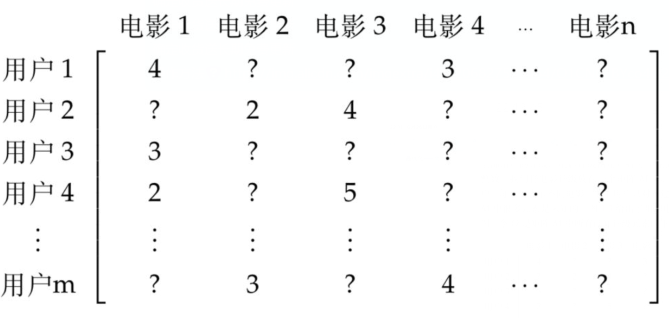
\includegraphics[scale=0.3]{1.png}
    \caption{用户电影评级系统}
    \end{figure}

列出优化问题
\begin{equation}
    \begin{aligned}
        min \ &rank(X) \\
        s.t. \ &X_{ij}=M_{ij}
    \end{aligned}
\end{equation}
其中$X$预测的结果矩阵,$M$是已知的矩阵值。仅有的约束条件就是$X$的部分值要与已知的值相等,
并且秩越低(越相似)越好。

但是求秩并不简单,$rank(X)$可以替换为非0奇异值个数。
根据稀疏优化的思想,可以更换为奇异值之和,也就是矩阵的核范数$||X||_*$。
问题(5)就变成了(6)
\begin{equation}
    \begin{aligned}
        min \ &||X||_* \\
        s.t. \ &X_{ij}=M_{ij} \ (i,j) \in \omega
    \end{aligned}
\end{equation}
很容易证明,问题(6)是一个凸优化的问题,也是半定规划问题。
它的二次罚函数形式为

\begin{equation}
    \begin{aligned}
        min \ \mu ||X||_* +\frac{1}{2}\sum_{(i,j)\in\omega}(X_{ij}-M_{ij})^2
    \end{aligned}
\end{equation}
%%%%%%%%%%%%%%%%%%%%%%%%%%%%%%%%%%%%%%%%%%%%%%%%%%%%%%%%%%%%%%%%%%%%%%%%%%%%%%%
%%%%%%%%%%%%%%%%%%%%%%%%%%%%%%%%%%%%%%%%%%%%%%%%%%%%%%%%%%%%%%%%%%%%%%%%%%%%%%%
%%%%%%%%%%%%%%%%%%%%%%%%%%%%%%%%%%%%%%%%%%%%%%%%%%%%%%%%%%%%%%%%%%%%%%%%%%%%%%%
\section{深度学习——多层感知机}

多层感知机(前馈神经网络、深度前馈网络)。
这里举例一个图片分类的神经网络,
比如说要区分是猫或者狗,就是在逼近一个从图片到$ \left\{ 0,1 \right\} $的函数。

具体的,给定一个训练集$D=\{ \{a_1,b_1\} , \{a_2,b_2\},...,\{ a_m,b_m\} \}$,
假设$a_i \in \mathbb{R}^p,b_i \in \mathbb{R}^q$,
并且设$a_i$的第一项是1,也就是$a_{i1}=1$。
$a_i$是输入,是输入层$l=0$,$b_i$是输出,是输出层$l=L+1$,中间还有$L$个隐藏层。

\begin{figure}[h]
    \centering
    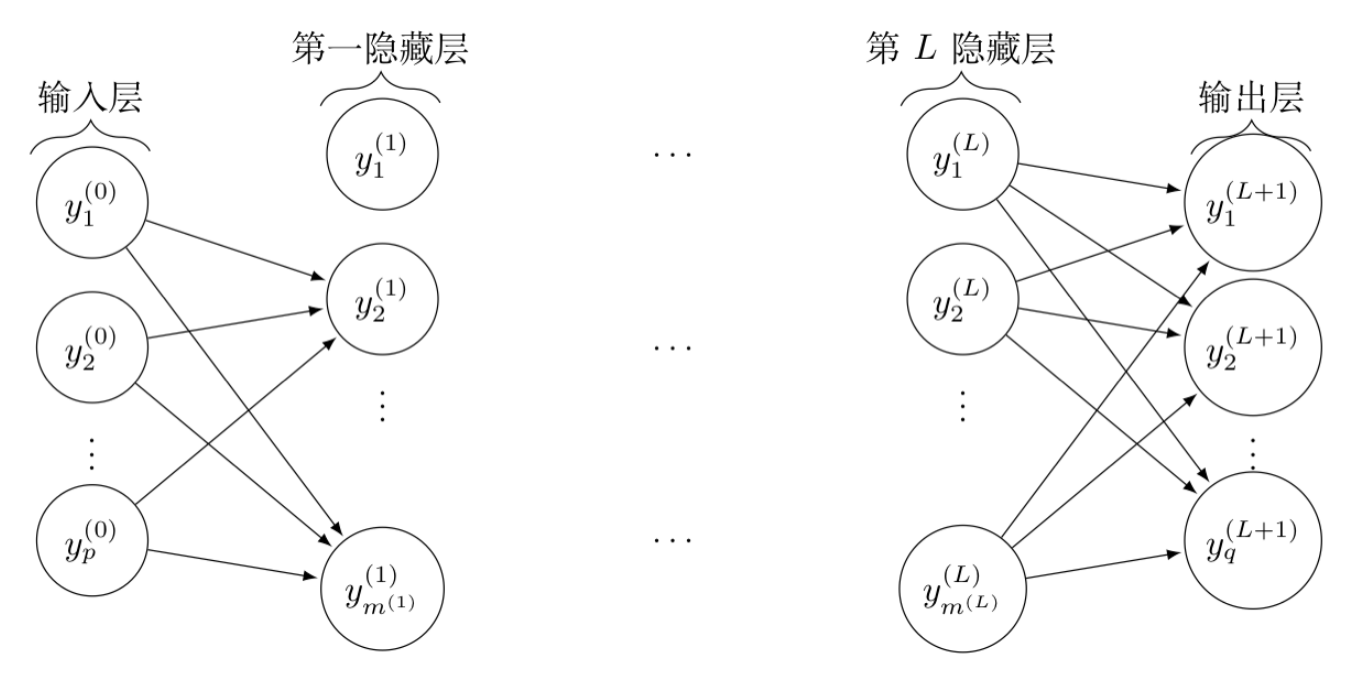
\includegraphics[scale=0.4]{2.png}
    \caption{神经网络结构}
    \end{figure}

多层感知机的实质就是由上一层的数值做线性组合再逐分量作线性变换得到的。
设第一层的元素为$y^{(0)}$,第二层的元素就是$y^{(1)}$,令它们的中间变量是$z^{(1)}$。
变换过程为:
\begin{equation}
    \begin{aligned}
  z^{(1)}_{(i)}=\sum_{k=1}^{p}x^{(l)}_{i,k}y^{(0)}_k 
    \end{aligned}
\end{equation}
这一步的$z^{(1)}$就是$y^{(0)}$中元素的简单加权求和。权重的选择未知。
下一步是把$z^{(1)}$变成$y^{(1)}$,这一步使用一个激活函数$t(\cdot)$
也就是
\begin{equation}
    \begin{aligned}
        y^{(1)}_i=t(z^{(1)})
    \end{aligned}
\end{equation}
激活函数$t(\cdot)$可以由很多函数,比如说Sigmoid函数
\begin{equation}
    \begin{aligned}
        t(z)=\frac{1}{1+exp(-z)} 
    \end{aligned}
\end{equation}
Heaviside函数
\begin{equation}
t(z)=\left\{ 
\begin{aligned}
    1,\ z \ge 0 \\ 
    0, \ z < 0 
\end{aligned}
\right.
\end{equation}
整个过程可以描述为
$y^{(0)} \rightarrow z^{(1)} \rightarrow y^{(1)} 
\rightarrow z^{(2)} \rightarrow y^{(2)} 
\rightarrow ... 
\rightarrow z^{(l)} \rightarrow y^{(l)}
\rightarrow z^{(l+1)} \rightarrow y^{(l+1)}$

那么多层感知机的优化模型就迟来了,为
\begin{equation}
    \mathop{min}\limits_x  \ \sum\limits_{i=1}^m ||h(a_i;x)-b_i||^2_2+\lambda r(x)
\end{equation}
其中$h(a_i;x)$是输出的结果,$b_i$是实际的结果,$r(x)$是正则项,用来刻画解的某些性质,
比如说稀疏性和光滑性。
%%%%%%%%%%%%%%%%%%%%%%%%%%%%%%%%%%%%%%%%%%%%%%%%%%%%%%%%%%%%%%%%%%%%%%%%%%%%%%%
%%%%%%%%%%%%%%%%%%%%%%%%%%%%%%%%%%%%%%%%%%%%%%%%%%%%%%%%%%%%%%%%%%%%%%%%%%%%%%%
%%%%%%%%%%%%%%%%%%%%%%%%%%%%%%%%%%%%%%%%%%%%%%%%%%%%%%%%%%%%%%%%%%%%%%%%%%%%%%%
\section{深度学习——卷积神经网络}
CNN,卷积神经网络,是一种深度前馈人工神经网络(前馈和反馈的区别),
可以用于时间序列和图像等网格数据的处理。

区别于上文中的多层感知机,卷积神经网络并没有采取全连接(即采用上一层中的所有数据),
仅选取部分数据,不过总体思想是一样的。
\begin{figure}[h]
    \centering
    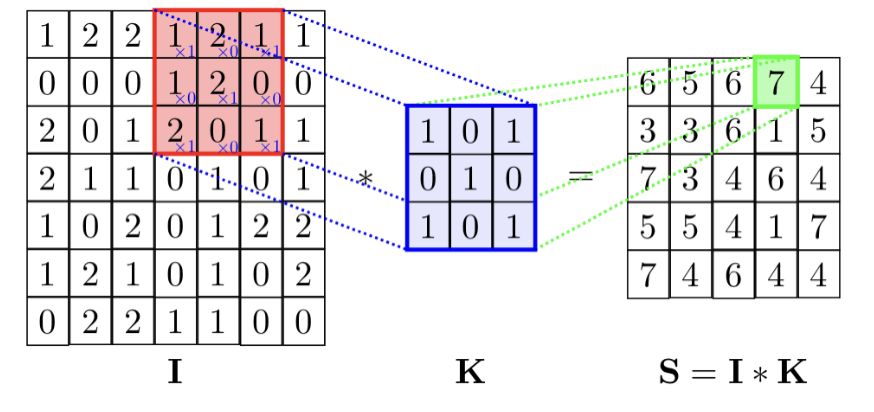
\includegraphics[scale=0.5]{3.png}
    \caption{卷积操作}
    \end{figure}
如图3所示,$K$是一个权重矩阵,取矩阵$I$中对应位置对应元素与权重矩阵$K$进行逐元素的相乘。
也就是说,给定一个二维图像$I \in \mathbb{R}^{n \times n}$以及卷积核$K \in \mathbb{R}^{k \times k}$。
有这样的一种卷积操作$S=I*K$,
并且每个元素满足式子$$ S_{i,j}=<I(i:i+k-1,j:j+k-1),K>$$

与多层感知机相似,整个流程也是输入图片,卷积(权重的赋值),激活函数,得到下一层。
以此类推,得到了卷积神经网络的结构,如图4所示。
\begin{figure}[h]
    \centering
    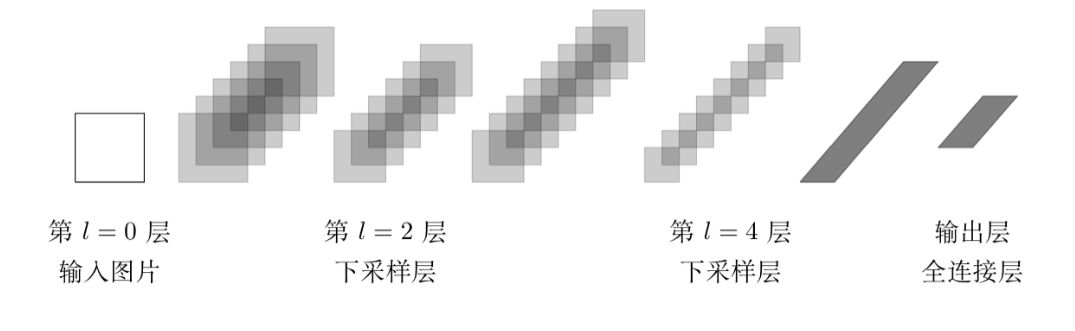
\includegraphics[scale=0.5]{4.png}
    \caption{卷积神经网络示意图}
    \end{figure}
%%%%%%%%%%%%%%%%%%%%%%%%%%%%%%%%%%%%%%%%%%%%%%%%%%%%%%%%%%%%%%%%%%%%%%%%%%%%%%%
%%%%%%%%%%%%%%%%%%%%%%%%%%%%%%%%%%%%%%%%%%%%%%%%%%%%%%%%%%%%%%%%%%%%%%%%%%%%%%%
%%%%%%%%%%%%%%%%%%%%%%%%%%%%%%%%%%%%%%%%%%%%%%%%%%%%%%%%%%%%%%%%%%%%%%%%%%%%%%%
\section{最优化基本概念}
主要任务(3个):\textbf{构造模型,确定优化问题设计算法,实现算法求解}。
%%%%%%%%%%%%%%%%%%%%%%%%%%%%%%%%%%%%%%%%%%%%%%%%%%%%%%%%%%%%%%%%%%%%%%%%%%%%%%%

连续和离散优化问题:
离散优化,变量在离散集合上取值(离散点集、整数集),比如说整数规划。
求解比较困难,一般需要把离散变成连续来求解(定界方法)。

有约束和无约束优化问题:
可以将约束罚到目标函数上去。
常见方法:\textbf{增广拉格朗日函数法、罚函数法}。

随机性和确定性优化问题:
随机优化问题:目标或者约束函数中涉及随机变量而带有不确定性的问题(只会这些参数的估计)。
在机器学习、强化学习有广泛的应用。
参数未知,所以实际中是通过足够大的样本,来逼近目标函数,得到一个有限和的目标函数。
以目标函数为多项求和的优化问题为例,使用确定性优化算法,会引入昂贵的复杂度。
但是对于随机优化问题,每次只能计算和式的一项或者几项,节约了计算时间。

线性规划和非线性规划问题:
46-47年单纯形法,79年线性规划问题多项式时间算法的存在,84年多项式时间的内点法。

凸和非凸优化问题:

全局最优解和局部最优解:全局极小解、严格局部最小解、非严格局部最小解。
\begin{figure}[h]
    \centering
    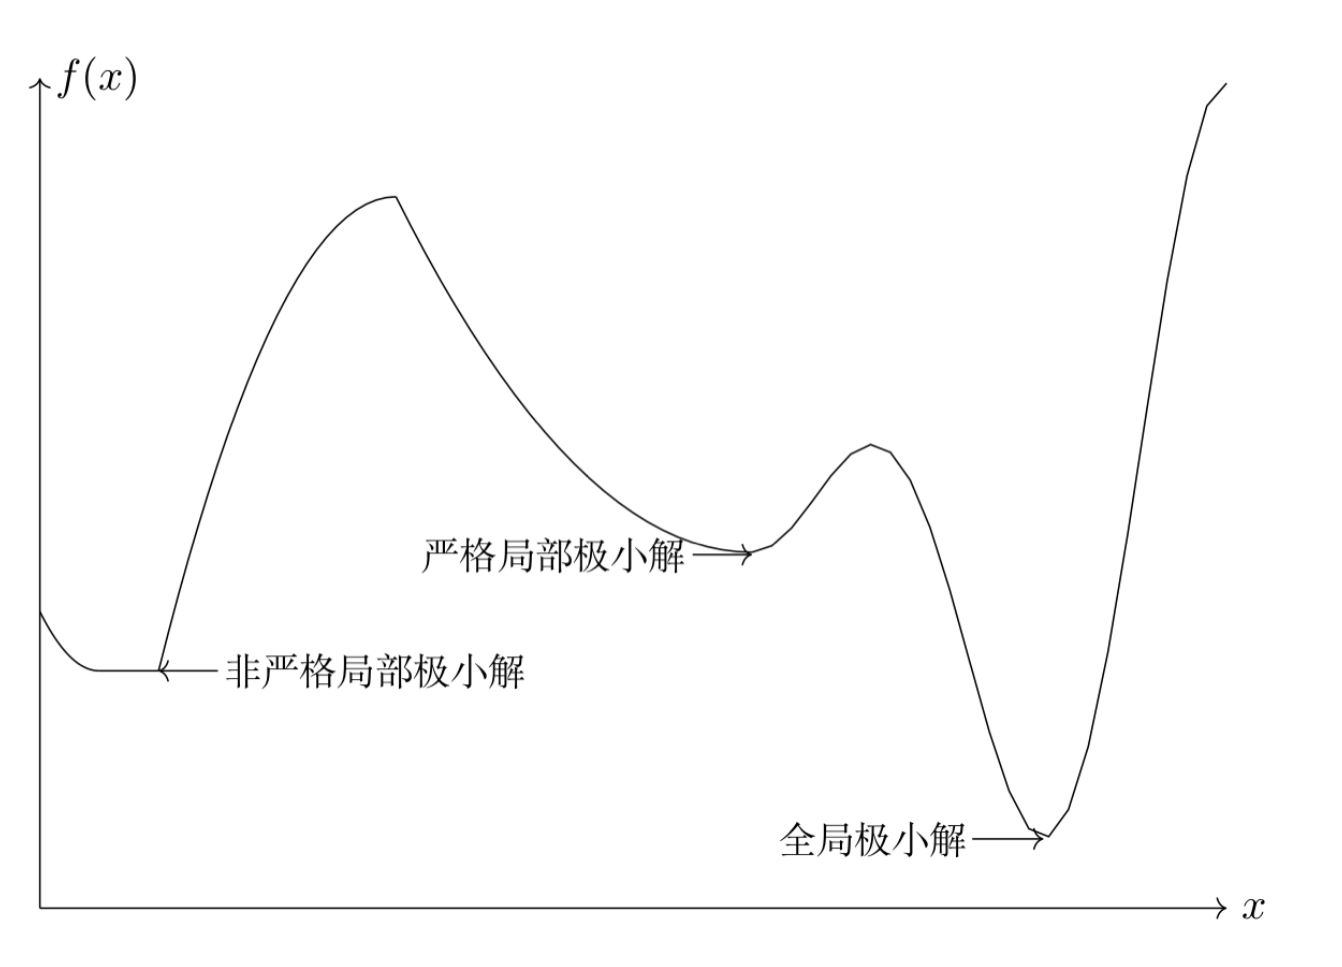
\includegraphics[scale=0.3]{5.png}
    \caption{全局极小解、严格局部最小解、非严格局部最小解}
    \end{figure}    
%%%%%%%%%%%%%%%%%%%%%%%%%%%%%%%%%%%%%%%%%%%%%%%%%%%%%%%%%%%%%%%%%%%%%%%%%%%%%%%
%%%%%%%%%%%%%%%%%%%%%%%%%%%%%%%%%%%%%%%%%%%%%%%%%%%%%%%%%%%%%%%%%%%%%%%%%%%%%%%
%%%%%%%%%%%%%%%%%%%%%%%%%%%%%%%%%%%%%%%%%%%%%%%%%%%%%%%%%%%%%%%%%%%%%%%%%%%%%%%
\section{最优化基本概念——优化算法}
能用代数表达式给出最优解——显式解,但是一般没法得到,就要用迭代算法。

那么迭代算法一定要有收敛准则,一般的收敛准则是
\begin{equation}
    \frac{f(x^k)-f^*}{max\{ |f^*|,1\}} \le \epsilon_1 ,\ ||\nabla f(x^k)|| \le \epsilon_2
\end{equation}
$\epsilon_1$和$\epsilon_2$都是很小的正数,$||*||$代表某种范数,$f^*$代表最优值。
也就是一般是用函数值或者梯度来判断收敛的。

除了收敛性还有违反约束度的分析。

还有与最优解之间的距离的分析。(此处省略)。

接下来是一些收敛的概念
\begin{table}[h]
    \centering
    \caption{一些概念}
    \begin{tabular}{|l|l|l|}\hline
    依点列收敛到局部(全局)极小解    &  从$x$角度来看收敛 \\ \hline
    全局依点列收敛到局部(全局)极小解  & 任意的初值$x0$  \\ \hline
    全局依函数值收敛到局部(全局)极小解 &  从$f(x)$角度来看收敛\\ \hline 
    \end{tabular}
\end{table}
除了点列和函数值的收敛,还会使用到如无约束优化问题中的梯度范数,有约束优化问题中的最优性违反度等.
%%%%%%%%%%%%%%%%%%%%%%%%%%%%%%%%%%%%%%%%%%%%%%%%%%%%%%%%%%%%%%%%%%%%%%%%%%%%%%%
%%%%%%%%%%%%%%%%%%%%%%%%%%%%%%%%%%%%%%%%%%%%%%%%%%%%%%%%%%%%%%%%%%%%%%%%%%%%%%%
\subsection{优化问题处理的操作技巧}
泰勒展开:对于一个非线性的目标函数或者约束函数,通过泰勒展开来用线性函数或者二次函数来逼近。
但是简化问题只在小邻域内逼近原始问题,需要不断根据迭代点来重新构造简化问题。

对偶:通过求解对偶问题来同时求解原始问题和对偶问题。(拉格朗日?)

拆分:如$\min\limits_{x} h(x)+g(x)$可以拆分为$\min \limits_{x,y} g(x)+h(y) \ \ s.t. \ x=y$
,这样通过交替求解来得到原问题的解。(ADMM算法)

块坐标下降:对于一个n维(n很大)空间的优化问题,通过逐步求解分量的方式来算。先固定$x_2-x_{100}$
去求解$x_1$,再固定$x_1$和$x_3-x_{100}$,求解$x_2$,以此类推。

\subsection{收敛速度Q和R}
对于充分大的$k$,Q收敛的定义为
\begin{table}[h]
    \centering
    \caption{Q收敛}
    \begin{tabular}{|l|l|l|}\hline
        \textbf{Q-线性收敛的}    &  $ \frac{||x^{k+1}-x^*||}{||x^{k}-x^*||} \le a,\ \ a \in (0,1)$\\ \hline
        \textbf{Q-超线性收敛的}  & $ \lim\limits_{k \rightarrow \infty}\frac{||x^{k+1}-x^*||}{||x^{k}-x^*||} =0$  \\ \hline
        \textbf{Q-次线性收敛的} &  $\lim\limits_{k \rightarrow \infty}\frac{||x^{k+1}-x^*||}{||x^{k}-x^*||} =1$\\ \hline 
        \textbf{Q-二次线性收敛的} &  $ \frac{||x^{k+1}-x^*||}{||x^{k}-x^*||^2} \le a,\ \ a \in (0,1)$\\ \hline 
    \end{tabular}
\end{table}

R收敛定义:以一个点列$\{x^k\}$为例,设$\{x^k\}$最终收敛到最优值$x^*$,并且存在一个非负序列$t_k$,使得$|x^k-x^*| \le t_k$,那么就称算法为\textbf{R线性收敛},同理还有\textbf{R超线性收敛}和\textbf{R二次收敛}。同时,这个非负序列还用于收敛速度计算上,成为$\mathbb{O}(t_k)$。此外,优化算法的复杂度$N(\epsilon)$,定义为计算出给定精度$\epsilon$的解所需的迭代次数或浮点运算次数,比如$f(x^k)-f(x^*) \le \epsilon$中的$k$的大小。复杂度与收敛速度之间息息相关,一个是从$x$的角度来看,一个是从$f(x)$的角度来看。

举例一个迭代序列$\{x^k\}$,满足$f(x^k)-f(x^*) \le \frac{c}{\sqrt{k}}, \ \forall k>0 $。得到$N(\epsilon)=\mathbb{O}(\frac{1}{\epsilon^2})$。

\section{小结}
本章主要讲了优化问题的基本概念以及分类、热点问题等。




\end{document}